\documentclass[11pt,a4paper]{article}

% --- Core Typography & Encoding ---
\usepackage[utf8]{inputenc}
\usepackage[T1]{fontenc}
\usepackage{lmodern}
\usepackage{microtype}

% --- Page Geometry ---
\usepackage[margin=20mm,top=25mm,bottom=25mm,footskip=12mm,headsep=10mm]{geometry}

% --- Math & Symbols ---
\usepackage{amsmath,amssymb,amsfonts,amsthm,mathtools}
\usepackage{bm}

% --- Tables & Figures ---
\usepackage{booktabs}
\usepackage{array}
\usepackage{tabularx}
\usepackage{multirow}
\usepackage{graphicx}
\usepackage{subcaption}
\usepackage{float}

% --- Colors ---
\usepackage[table,xcdraw,dvipsnames]{xcolor}
\definecolor{foamNavy}{RGB}{15, 44, 89}
\definecolor{foamBlue}{RGB}{24, 77, 140}
\definecolor{foamTeal}{RGB}{0, 136, 170}
\definecolor{foamDark}{RGB}{33, 37, 41}
\definecolor{foamLight}{RGB}{248, 250, 252}
\definecolor{foamBorder}{RGB}{226, 232, 240}
\definecolor{codeBg}{RGB}{245, 247, 250}
\definecolor{codeFrame}{RGB}{209, 217, 230}
\definecolor{alertRed}{RGB}{185, 28, 28}
\definecolor{tipGreen}{RGB}{22, 101, 52}
\definecolor{warnAmber}{RGB}{180, 83, 9}

% --- TikZ & Diagrams ---
\usepackage{tikz}
\usetikzlibrary{shapes,arrows.meta,positioning,calc,fit,backgrounds,decorations.pathreplacing}

% --- Code Listings ---
\usepackage{listings}
\lstset{
    language=C++,
    basicstyle=\ttfamily\footnotesize\color{foamDark},
    keywordstyle=\bfseries\color{foamNavy},
    commentstyle=\itshape\color{gray},
    stringstyle=\color{tipGreen},
    numbers=left,
    numberstyle=\tiny\color{gray},
    stepnumber=1,
    numbersep=8pt,
    backgroundcolor=\color{codeBg},
    frame=single,
    rulecolor=\color{codeFrame},
    tabsize=4,
    showspaces=false,
    showstringspaces=false,
    breaklines=true,
    breakatwhitespace=true,
    captionpos=b,
    xleftmargin=15pt,
    framexleftmargin=15pt
}

% --- Fancy Header & Footer ---
\usepackage{fancyhdr}
\pagestyle{fancy}
\fancyhf{}
\fancyhead[L]{\small\color{gray}\textbf{freeFallingFoam} \textbullet\ Developer \& Physics Architecture Guide}
\fancyhead[R]{\small\color{gray}\thepage}
\fancyfoot[C]{\footnotesize\color{gray}OpenFOAM\textregistered\ Custom Solver Suite --- Internal Engineering Documentation}
\renewcommand{\headrulewidth}{0.4pt}
\renewcommand{\footrulewidth}{0.4pt}

% --- Callout Boxes (tcolorbox) ---
\usepackage[most]{tcolorbox}
\newtcolorbox{infobox}[1][]{
    enhanced,
    colback=foamLight,
    colframe=foamBlue,
    fonttitle=\bfseries\color{white},
    coltitle=white,
    colbacktitle=foamBlue,
    title=#1,
    arc=3mm,
    boxrule=1pt,
    left=4mm,right=4mm,top=3mm,bottom=3mm,
    drop shadow=black!10
}
\newtcolorbox{warningbox}[1][]{
    enhanced,
    colback=red!5!white,
    colframe=alertRed,
    fonttitle=\bfseries\color{white},
    coltitle=white,
    colbacktitle=alertRed,
    title=#1,
    arc=3mm,
    boxrule=1pt,
    left=4mm,right=4mm,top=3mm,bottom=3mm,
    drop shadow=black!10
}
\newtcolorbox{tipbox}[1][]{
    enhanced,
    colback=green!5!white,
    colframe=tipGreen,
    fonttitle=\bfseries\color{white},
    coltitle=white,
    colbacktitle=tipGreen,
    title=#1,
    arc=3mm,
    boxrule=1pt,
    left=4mm,right=4mm,top=3mm,bottom=3mm,
    drop shadow=black!10
}
\newtcolorbox{theorybox}[1][]{
    enhanced,
    colback=foamLight,
    colframe=foamNavy,
    fonttitle=\bfseries\color{white},
    coltitle=white,
    colbacktitle=foamNavy,
    title=#1,
    arc=3mm,
    boxrule=1.2pt,
    left=4mm,right=4mm,top=3mm,bottom=3mm,
    drop shadow=black!12
}

% --- Hyperlinks ---
\usepackage{hyperref}
\hypersetup{
    colorlinks=true,
    linkcolor=foamNavy,
    citecolor=foamTeal,
    urlcolor=foamBlue,
    pdfauthor={freeFallingFoam Core Architecture Team},
    pdftitle={freeFallingFoam Solver Architecture and Physics Manual},
    pdfsubject={Developer Documentation for Accelerating Reference Frames and 6DoF Dynamics in OpenFOAM}
}

% --- Custom Math Operators ---
\newcommand{\vect}[1]{\mathbf{#1}}
\newcommand{\tensor}[1]{\bm{#1}}
\newcommand{\grad}{\nabla}
\newcommand{\pderiv}[2]{\frac{\partial #1}{\partial #2}}
\newcommand{\dderiv}[2]{\frac{\mathrm{d} #1}{\mathrm{d} #2}}
\newcommand{\Dderiv}[2]{\frac{\mathrm{D} #1}{\mathrm{D} #2}}
\newcommand{\prgh}{p_{\mathrm{rgh}}}
\newcommand{\aframe}{\vect{a}_{\mathrm{frame}}}
\newcommand{\vframe}{\vect{V}_{\mathrm{frame}}}
\newcommand{\faero}{\vect{F}_{\mathrm{aero}}}
\newcommand{\fgrav}{\vect{F}_{\mathrm{grav}}}
\newcommand{\fapp}{\vect{f}_{\mathrm{app}}}
\newcommand{\maero}{\vect{M}_{\mathrm{aero}}}
\newcommand{\omegab}{\bm{\omega}_b}

% ============================================================================
%  DOCUMENT BEGIN
% ============================================================================
\begin{document}

% --- Title Page ---
\begin{titlepage}
    \centering
    \vspace*{1.0cm}
    
    {\Huge \bfseries \color{foamNavy} freeFallingFoam}\\[0.4cm]
    {\LARGE \bfseries \color{foamBlue} Architecture, Physics, and Developer Onboarding Guide}\\[0.6cm]
    {\large \color{foamDark} A Comprehensive Handbook for Junior CFD Developers on Body-Fixed Accelerating Frames, 6DoF Tumbling Dynamics, and Fluid-Structure Coupling in OpenFOAM}
    
    \vspace{1.2cm}
    \begin{tikzpicture}
        \draw[line width=1.5pt, color=foamTeal] (0,0) -- (10,0);
        \node[fill=foamLight, draw=foamNavy, line width=1pt, rounded corners=3pt, inner sep=5pt, text width=13cm, text centered] at (5,0) 
            {\bfseries\small\color{foamNavy} CORE OPENFOAM SOLVER SUITE:\\freeBodyPimpleFoam \textbullet\ freeBodyRhoPimpleFoam \textbullet\ freeBodyRhoCentralFoam \textbullet\ freeBody6DoFPimpleFoam};
    \end{tikzpicture}
    \vspace{0.8cm}

    % Central Schematic Preview
    \begin{figure}[H]
        \centering
        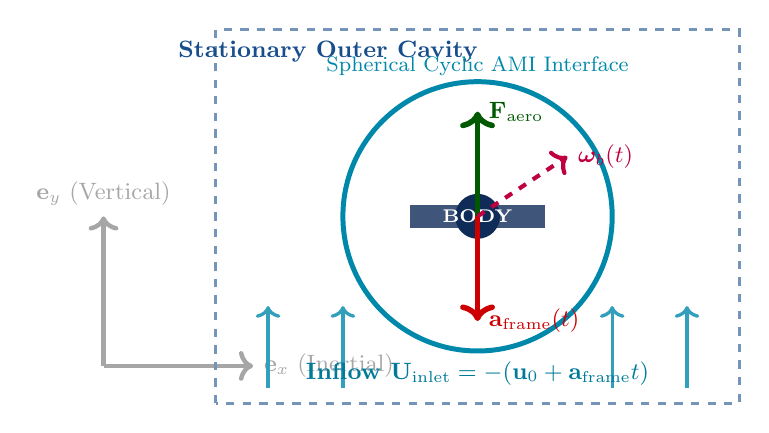
\begin{tikzpicture}[scale=0.95, every node/.style={transform shape}]
            % World frame
            \draw[->, ultra thick, color=gray!70] (-5,-2) -- (-3,-2) node[right] {\small $\vect{e}_x$ (Inertial)};
            \draw[->, ultra thick, color=gray!70] (-5,-2) -- (-5,0) node[above] {\small $\vect{e}_y$ (Vertical)};
            
            % Falling Domain Outer Box
            \draw[dashed, line width=1.2pt, color=foamBlue!60] (-3.5,-2.5) rectangle (3.5,2.5);
            \node[color=foamBlue, font=\bfseries\small] at (-2.0,2.2) {Stationary Outer Cavity};
            
            % Spherical AMI
            \draw[line width=1.8pt, color=foamTeal] (0,0) circle (1.8cm);
            \node[color=foamTeal, font=\footnotesize] at (0, 2.0) {Spherical Cyclic AMI Interface};
            
            % Body in center
            \fill[color=foamNavy!80] (-0.9,-0.15) rectangle (0.9,0.15);
            \fill[color=foamNavy] (0,0) circle (0.3cm);
            \node[color=white, font=\bfseries\scriptsize] at (0,0) {BODY};
            
            % Kinematic Vectors
            \draw[->, line width=2pt, color=red!80!black] (0,0) -- (0,-1.4) node[right, font=\bfseries\small] {$\aframe(t)$};
            \draw[->, line width=2pt, color=Green!70!black] (0,0) -- (0,1.4) node[right, font=\bfseries\small] {$\faero$};
            \draw[->, line width=1.5pt, color=purple, dashed] (0,0) -- (1.2,0.8) node[right, font=\bfseries\small] {$\omegab(t)$};
            
            % Relative Freestream Inflow
            \foreach \x in {-2.8, -1.8, 1.8, 2.8} {
                \draw[->, line width=1.2pt, color=foamTeal!80] (\x, -2.3) -- (\x, -1.2);
            }
            \node[color=foamTeal!90!black, font=\bfseries\small] at (0, -2.1) {Inflow $\vect{U}_{\mathrm{inlet}} = -(\vect{u}_0 + \aframe t)$};
        \end{tikzpicture}
    \end{figure}

    \vfill
    
    \begin{tcolorbox}[colback=foamLight, colframe=foamNavy!30, arc=2mm, width=0.88\textwidth]
        \centering\small\color{foamDark}
        \textbf{Document Version:} 2.4.0 \textbullet\ \textbf{Compatibility:} OpenFOAM v2006 -- v2412\\
        \textbf{Primary Maintainer:} Senior CFD Systems Engineering Team\\
        \textbf{Target Audience:} Incoming Postgraduates, CFD Research Engineers, and Junior Developers
    \end{tcolorbox}
    
    \vspace{0.4cm}
    {\small \color{gray} Compiled: \today}
\end{titlepage}

\newpage
\tableofcontents
\newpage

% ============================================================================
%  SECTION 1: ONBOARDING & EXECUTIVE SUMMARY
% ============================================================================
\section{Welcome \& Executive Orientation}

\subsection{Why Does \texttt{freeFallingFoam} Exist?}
Welcome to the team! If you are reading this manual, your task is to understand, maintain, debug, or extend the \texttt{freeFallingFoam} solver suite. 

Before touching a single line of C++, you must understand the primary computational bottleneck that motivated the creation of this solver. 
In traditional Computational Fluid Dynamics (CFD), when modeling an object falling under gravity (such as an atmospheric re-entry capsule, a projectile, an autorotating seed, or a tumbling propeller), engineers face an immediate dilemma:
\begin{enumerate}
    \item \textbf{The Stationary Domain Trap:} If the simulation domain covers the full trajectory (e.g., $10\text{ km}$ of free-fall altitude), the computational mesh must contain trillions of cells, or suffer from severe numerical diffusion due to coarse cell sizes across kilometers of air.
    \item \textbf{The Translating Mesh Trap:} If the mesh dynamically translates down a coordinate axis along with the body, boundary layers on outer domain boundaries create artificial shear, mesh deformation algorithms risk element inversion, and coordinate precision degrades over large spatial displacements.
\end{enumerate}

\begin{theorybox}[The Governing Innovation: The Body-Fixed Accelerating Frame]
Instead of translating the mesh through the sky, \texttt{freeFallingFoam} fixes the coordinate system directly to the falling body. 
The body remains permanently centered at $(0, 0, 0)$ in the computational domain.
The downward acceleration of the body $\aframe(t)$ is formulated mathematically as an \textbf{apparent inertial body force} (d'Alembert fictitious force) injected into the momentum equations, while the relative freestream air rushing past the body is prescribed dynamically on the domain boundaries.
\end{theorybox}

This approach yields monumental computational advantages:
\begin{itemize}
    \item \textbf{Extreme Mesh Efficiency:} The computational mesh only needs to resolve the immediate vicinity and turbulent wake of the body (typically a bounding box of $10$ to $50$ body diameters).
    \item \textbf{Infinite Fall Duration:} The body can fall from orbit through the entire stratosphere to sea level ($100\text{ km} \to 0\text{ km}$) within a fixed, compact mesh.
    \item \textbf{Exact Conservation:} The boundary layer surrounding the body remains topologically pristine throughout the simulation without mesh stretching or morphing degradation.
\end{itemize}

\subsection{Architectural Decoupling: Translation vs. Rotation}
A core engineering breakthrough implemented in \texttt{freeBody6DoFPimpleFoam} is the \textbf{decoupling of translational and rotational kinematics}:
\begin{itemize}
    \item \textbf{Translation is absorbed by the accelerating reference frame.} The frame does \emph{not} rotate with the body; it only accelerates linearly. Consequently, there are \textbf{zero fictitious Coriolis} ($-2\bm{\omega}\times\vect{U}$) and \textbf{zero centrifugal} ($-\bm{\omega}\times(\bm{\omega}\times\vect{r})$) body force fields in the Navier-Stokes equations!
    \item \textbf{Rotation is resolved physically by an inner spherical mesh.} The body is enclosed within a spherical rotary sub-domain that rotates physically across an Arbitrary Mesh Interface (\texttt{cyclicAMI}) relative to a matching outer spherical cavity.
\end{itemize}

\begin{figure}[H]
    \centering
    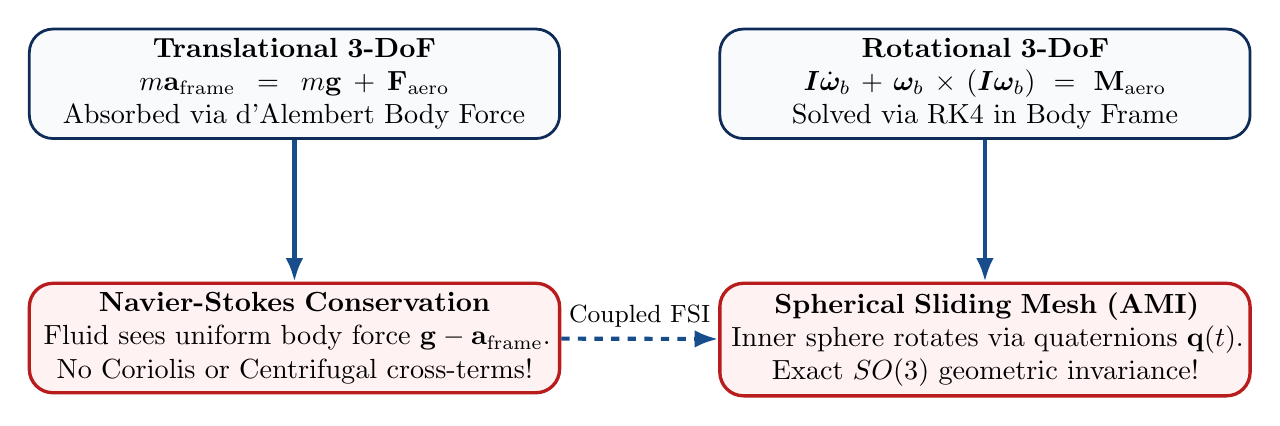
\begin{tikzpicture}[node distance=2.2cm, auto, >=Latex]
        \tikzstyle{block} = [rectangle, draw=foamNavy, fill=foamLight, text width=6.5cm, text centered, rounded corners=3mm, minimum height=1.3cm, line width=1pt]
        \tikzstyle{highlight} = [rectangle, draw=alertRed, fill=red!5!white, text width=6.5cm, text centered, rounded corners=3mm, minimum height=1.3cm, line width=1.2pt]
        \tikzstyle{line} = [draw=foamBlue, -{Latex[length=3mm]}, line width=1.5pt]

        \node [block] (trans) {\textbf{Translational 3-DoF}\\$\displaystyle m\aframe = m\vect{g} + \faero$\\Absorbed via d'Alembert Body Force};
        \node [block, right=2cm of trans] (rot) {\textbf{Rotational 3-DoF}\\$\displaystyle \tensor{I}\dot{\bm{\omega}}_b + \bm{\omega}_b\times(\tensor{I}\bm{\omega}_b) = \maero$\\Solved via RK4 in Body Frame};
        \node [highlight, below=1.8cm of trans] (fsi) {\textbf{Navier-Stokes Conservation}\\Fluid sees uniform body force $\vect{g} - \aframe$.\\No Coriolis or Centrifugal cross-terms!};
        \node [highlight, below=1.8cm of rot] (mesh) {\textbf{Spherical Sliding Mesh (AMI)}\\Inner sphere rotates via quaternions $\vect{q}(t)$.\\Exact $SO(3)$ geometric invariance!};

        \path [line] (trans) -- (fsi);
        \path [line] (rot) -- (mesh);
        \path [line, dashed] (fsi) -- node[above] {\small Coupled FSI} (mesh);
    \end{tikzpicture}
    \caption{The decoupled translational-rotational architecture in \texttt{freeFallingFoam}.}
    \label{fig:decoupled_arch}
\end{figure}

% ============================================================================
%  SECTION 2: MATHEMATICAL & PHYSICAL FORMULATION
% ============================================================================
\section{Mathematical \& Physical Foundations}

As a junior developer modifying this solver, you must understand the exact coordinate transformations and continuum mechanics equations implemented in the code. Never alter \texttt{UEqn.H} or \texttt{pEqn.H} without consulting this section.

\subsection{Coordinate Systems \& Transformation Kinematics}
Let $(\vect{E}_X, \vect{E}_Y, \vect{E}_Z)$ denote a fixed, right-handed \textbf{Inertial Reference Frame} $\mathcal{F}_I$ attached to the Earth (neglecting planetary rotation for local trajectory scales). 
Let $\mathcal{F}_{\mathrm{frame}}$ be a non-rotating, accelerating reference frame whose origin $\vect{R}(t)$ is tied to the center of mass of the falling projectile.

The position vector $\vect{r}_I$ of an arbitrary fluid packet in the inertial frame is given by:
\begin{equation}
    \vect{r}_I(t) = \vect{R}(t) + \vect{r}(t)
\end{equation}
where $\vect{r}(t)$ is the position vector measured in the body-fixed accelerating frame.

Differentiating with respect to time:
\begin{align}
    \vect{v}_I(t) &= \dderiv{\vect{R}}{t} + \dderiv{\vect{r}}{t} = \vframe(t) + \vect{U}(\vect{r}, t) \\
    \vect{a}_I(t) &= \dderiv{\vframe}{t} + \Dderiv{\vect{U}}{t} = \aframe(t) + \left[ \pderiv{\vect{U}}{t} + (\vect{U} \cdot \grad)\vect{U} \right]
\end{align}
where $\vect{U}$ is the fluid velocity vector \emph{relative to the falling frame}.

\subsection{Derivation of the Non-Inertial Momentum Equation}
The Cauchy momentum equation in the inertial frame is:
\begin{equation}
    \rho \vect{a}_I = -\grad p_I + \grad \cdot \tensor{\tau} + \rho \vect{g}
\end{equation}
Substituting the kinematic acceleration of the accelerating frame:
\begin{equation}
    \rho \left[ \pderiv{\vect{U}}{t} + (\vect{U} \cdot \grad)\vect{U} + \aframe \right] = -\grad p + \grad \cdot \tensor{\tau} + \rho \vect{g}
\end{equation}
Rearranging to place all convective terms on the left and forcing terms on the right:
\begin{equation}
    \boxed{\rho \left[ \pderiv{\vect{U}}{t} + \grad \cdot (\vect{U} \otimes \vect{U}) \right] = -\grad p + \grad \cdot \tensor{\tau} + \rho (\vect{g} - \aframe)}
    \label{eq:navier_stokes_accel}
\end{equation}
where:
\begin{itemize}
    \item $\vect{g}$ is the planetary gravitational acceleration vector (typically $(0, -9.81, 0)\text{ m/s}^2$).
    \item $\aframe$ is the instantaneous kinematic acceleration of the falling body.
    \item $\fapp \equiv \vect{g} - \aframe$ is the \textbf{apparent net body force} experienced by the fluid.
\end{itemize}

\subsection{Physical Limiting Cases of the Apparent Body Force}
Equation~\eqref{eq:navier_stokes_accel} reveals profound physical elegance when examining the life cycle of a falling body:

\begin{theorybox}[Physical Limiting States of $\fapp$]
\begin{enumerate}
    \item \textbf{Vacuum Free Fall (Zero Drag, $t = 0$):}\\
    When released from rest in a vacuum or at the very first instant of release where $\vect{U}_{\mathrm{rel}} = 0$, aerodynamic drag is zero. 
    By Newton's second law for the body:
    \begin{equation}
        m\aframe = m\vect{g} \implies \aframe = \vect{g}
    \end{equation}
    Therefore:
    \begin{equation}
        \fapp = \vect{g} - \aframe = \vect{g} - \vect{g} = \vect{0}
    \end{equation}
    \textbf{Physical Meaning:} In free fall, the fluid inside the computational domain experiences \textbf{apparent weightlessness} (zero effective gravity), precisely as an astronaut does inside the International Space Station or a drop tower!
    
    \item \textbf{Terminal Velocity ($t \to \infty$):}\\
    As the body accelerates downward, aerodynamic drag increases until it exactly balances gravity:
    \begin{equation}
        m\aframe = m\vect{g} + \faero = \vect{0} \implies \aframe = \vect{0}
    \end{equation}
    Therefore:
    \begin{equation}
        \fapp = \vect{g} - \vect{0} = \vect{g}
    \end{equation}
    \textbf{Physical Meaning:} At terminal velocity, frame acceleration vanishes. The apparent body force smoothly recovers the standard terrestrial hydrostatic gravity vector $\vect{g}$!
\end{enumerate}
\end{theorybox}

\subsection{The Reduced Pressure Formulation (\texorpdfstring{$\prgh$}{p\_rgh})}
\label{sec:prgh_formulation}
In incompressible OpenFOAM solvers, numerical stability demands that hydrostatic pressure gradients be decoupled from the dynamic pressure.
In our accelerating reference frame, the effective body force is $\fapp = \vect{g} - \aframe$.

The total static pressure gradient is decomposed as:
\begin{equation}
    \grad p = \grad \prgh + \rho \fapp = \grad \prgh + \rho (\vect{g} - \aframe)
\end{equation}
Integrating spatially yields the definition of the reduced pressure field $\prgh$:
\begin{equation}
    \boxed{\prgh = p - \rho \left( \fapp \cdot \vect{r} \right) = p - \rho \left[ (\vect{g} - \aframe) \cdot \vect{r} \right]}
\end{equation}
where $\vect{r} = \vect{C}$ represents the cell center position vector relative to the coordinate origin.

\begin{warningbox}[CRITICAL DEVELOPER WARNING: Why $\prgh$ is Mandatory for 6DoF Solvers]
Do not attempt to rewrite \texttt{freeBody6DoFPimpleFoam} to solve directly for raw pressure $p$!
If a non-spherical or asymmetric body rotates in an accelerating frame, the uniform body force $\rho(\vect{g} - \aframe)$ creates a spatial hydrostatic pressure gradient across the domain.
If you compute surface aerodynamic forces by integrating raw pressure $p$, any slight geometric asymmetry introduces an artificial buoyant force and moment that scales with the domain bounds, causing numerical instability and catastrophic rotational divergence!
Working with $\prgh$ removes the pseudo-hydrostatic field, isolating the \textbf{true aerodynamic forces and moments}.
\end{warningbox}

\subsubsection{Dynamic Pressure Reset During Acceleration Updates}
Because $\aframe(t)$ varies from timestep to timestep, the spatial definition of $\prgh$ shifts dynamically:
\begin{equation}
    \prgh^{n+1} = \prgh^n + \rho \left( \fapp^n \cdot \vect{r} - \fapp^{n+1} \cdot \vect{r} \right)
\end{equation}
In the source code (\texttt{predictFallingFrameMotion.H} and \texttt{correctFallingFrameMotion.H}), this appears as:
\begin{lstlisting}
const volScalarField gh_old("gh_old", gh);
gh = (fallingFrameForce & mesh.C());
ghf = (fallingFrameForce & mesh.Cf());
p_rgh += gh_old - gh;
\end{lstlisting}
This discrete field adjustment preserves pressure continuity across kinematic updates!

\subsection{Atmospheric Stratification \& Environmental Physics}
Real projectiles and falling bodies fall through stratified planetary atmospheres. \texttt{freeFallingFoam} natively supports continuous atmospheric variation via runtime-selectable models:

\begin{enumerate}
    \item \textbf{Barometric Exponential Density ($\rho(z)$):}
    \begin{equation}
        \rho_{\mathrm{atm}}(z) = \rho_0 \exp\left( -\frac{\max(z - z_{\mathrm{ground}}, 0)}{H_{\mathrm{scale}}} \right)
    \end{equation}
    where $\rho_0$ is sea-level air density ($1.204\text{ kg/m}^3$ default), $H_{\mathrm{scale}} \approx 8400\text{ m}$ is the Earth atmospheric scale height, and $z$ is the tracked simulation altitude.
    
    \item \textbf{Altitude-Dependent Gravity ($g(z)$):}
    \begin{equation}
        \vect{g}(z) = \vect{g}_0 \left( \frac{R_E}{R_E + \max(z - z_{\mathrm{ground}}, 0)} \right)^2
    \end{equation}
    where $R_E = 6.371 \times 10^6\text{ m}$ is Earth's mean radius.
    
    \item \textbf{Mean Atmospheric Wind Profile ($\vect{U}_{\mathrm{mean}}(z)$):}
    The runtime-selectable \texttt{meanFlowModel} provides horizontal cross-winds, atmospheric boundary layer shear profiles ($z/z_0)^\alpha$, or tabulated sounding data.
\end{enumerate}

\subsection{The Custom Boundary Condition: \texttt{fallingInletVelocity}}
The relative velocity entering the computational domain must mirror the instantaneous velocity of the falling frame plus any prevailing ambient wind:
\begin{equation}
    \vect{U}_{\mathrm{rel}}(t) = \vect{U}_{\mathrm{mean}}(z) - \vframe(t)
\end{equation}

The custom boundary condition \texttt{fallingInletVelocity} implements a \textbf{directionally-adaptive mixed Dirichlet/Neumann condition}:
\begin{equation}
    \vect{U}_{\mathrm{patch}} = 
    \begin{cases}
        \vect{U}_{\mathrm{rel}} & \text{if } \vect{S}_f \cdot \vect{U}_{\mathrm{test}} < -\epsilon \quad \text{(Inflow Face: Dirichlet)} \\
        \grad \vect{U} \cdot \vect{n} = \vect{0} & \text{if } \vect{S}_f \cdot \vect{U}_{\mathrm{test}} \ge -\epsilon \quad \text{(Outflow Face: Neumann)}
    \end{cases}
\end{equation}
where $\vect{S}_f$ is the outward-pointing face area vector.

\begin{tipbox}[Why Mixed Inflow/Outflow Matters]
As a body tumbles or drifts laterally due to crosswinds, the inflow and outflow faces of the bounding box rotate and shift dynamically. 
The zero-gradient Neumann condition on outflow faces allows turbulent wake vortices, shear layers, and acoustic pressure waves to leave the domain smoothly without artificial wall reflections.
\end{tipbox}

% ============================================================================
%  SECTION 3: 6DOF DYNAMICS & ROTATIONAL MECHANICS
% ============================================================================
\section{6DoF Rotational Dynamics \& Spherical Sliding Mesh}

Simulating tumbling bodies (such as the 10-inch propeller in \texttt{propTumble}) introduces complex rotational physics. This section explains how 6DoF rotation is formulated and solved.

\subsection{Rigid Body Rotational Equations of Motion}
Rotational motion is governed by Euler's equations formulated in the \textbf{body-fixed principal axis frame} where the mass moment of inertia tensor is purely diagonal:
\begin{equation}
    \tensor{I}_b = 
    \begin{bmatrix}
        I_{xx} & 0 & 0 \\
        0 & I_{yy} & 0 \\
        0 & 0 & I_{zz}
    \end{bmatrix}
\end{equation}
Euler's equations for the principal angular velocity vector $\omegab = (\omega_x, \omega_y, \omega_z)^T$ are:
\begin{equation}
    \boxed{
    \begin{aligned}
        I_{xx} \dderiv{\omega_x}{t} + (I_{zz} - I_{yy}) \omega_y \omega_z &= M_{b,x} \\
        I_{yy} \dderiv{\omega_y}{t} + (I_{xx} - I_{zz}) \omega_z \omega_x &= M_{b,y} \\
        I_{zz} \dderiv{\omega_z}{t} + (I_{yy} - I_{xx}) \omega_x \omega_y &= M_{b,z}
    \end{aligned}
    }
    \label{eq:euler_rotation}
\end{equation}
where $\vect{M}_b$ is the total external aerodynamic moment projected into the body principal axes.

\subsection{Aerodynamic Force and Moment Surface Integration}
At each CFD time step, \texttt{freeBody6DoFPimpleFoam} integrates the converged surface pressure and viscous shear stress over all specified wall patches (e.g., \texttt{propeller}):
\begin{align}
    \vect{F}_{\mathrm{press}} &= \sum_{\mathrm{faces}} \prgh \vect{S}_f \rho_{\mathrm{atm}} \\
    \vect{F}_{\mathrm{visc}}  &= \sum_{\mathrm{faces}} (\tensor{\tau}_{\mathrm{wall}} \cdot \vect{S}_f) \rho_{\mathrm{atm}} \\
    \maero &= \sum_{\mathrm{faces}} (\vect{C}_f - \vect{r}_{\mathrm{hub}}) \times \left( \mathrm{d}\vect{F}_{\mathrm{press}} + \mathrm{d}\vect{F}_{\mathrm{visc}} \right)
\end{align}
where $\vect{C}_f$ is the face centroid, $\vect{r}_{\mathrm{hub}}$ is the center of mass origin, and $\tensor{\tau}_{\mathrm{wall}} = \texttt{devReff()}$.

The total moment in world coordinates $\maero$ is then transformed into the body frame via the transpose of the attitude rotation matrix $\tensor{R}$:
\begin{equation}
    \vect{M}_b = \tensor{R}^T \maero
\end{equation}

\subsection{Fourth-Order Runge-Kutta (RK4) ODE Integration}
Euler's non-linear equations~\eqref{eq:euler_rotation} are integrated across the time step $\Delta t$ using a 4th-order Runge-Kutta (RK4) sub-stepper:
\begin{equation}
    \dderiv{\omegab}{t} = \vect{f}(\omegab) = \tensor{I}_b^{-1} \left( \vect{M}_b - \omegab \times (\tensor{I}_b \omegab) \right)
\end{equation}
The discrete RK4 stages are evaluated in \texttt{correctRotorDynamics.H}:
\begin{equation}
    \begin{aligned}
        \vect{k}_1 &= \vect{f}(\omegab^n) \\
        \vect{k}_2 &= \vect{f}\left(\omegab^n + \tfrac{1}{2}\Delta t \vect{k}_1\right) \\
        \vect{k}_3 &= \vect{f}\left(\omegab^n + \tfrac{1}{2}\Delta t \vect{k}_2\right) \\
        \vect{k}_4 &= \vect{f}(\omegab^n + \Delta t \vect{k}_3) \\
        \omegab^{n+1} &= \omegab^n + \frac{\Delta t}{6} \left( \vect{k}_1 + 2\vect{k}_2 + 2\vect{k}_3 + \vect{k}_4 \right)
    \end{aligned}
\end{equation}

\subsection{Singularity-Free Attitude Quaternions}
To prevent mathematical gimbal lock during arbitrary multi-turn 3D tumbling, the body attitude is tracked using a \textbf{unit quaternion} $\vect{q} = (w, \vect{v}) = (w, x, y, z) \in \mathbb{H}$.

Given the converged body angular velocity $\omegab^{n+1}$, the incremental attitude rotation quaternion $\Delta \vect{q}$ over time step $\Delta t$ is computed via the exponential map:
\begin{equation}
    \theta = \|\omegab\|\Delta t, \quad \vect{u} = \frac{\omegab}{\|\omegab\|}
\end{equation}
\begin{equation}
    \Delta \vect{q} = \left( \cos\frac{\theta}{2}, \ \vect{u} \sin\frac{\theta}{2} \right)
\end{equation}
The body attitude is updated via quaternion Hamilton product and normalized:
\begin{equation}
    \vect{q}^{n+1} = \vect{q}^n \otimes \Delta \vect{q}, \qquad \vect{q}^{n+1} \leftarrow \frac{\vect{q}^{n+1}}{\|\vect{q}^{n+1}\|}
\end{equation}

\subsection{The Intermediate Axis Theorem (The Dzhanibekov Phenomenon)}
For a solid Nylon PA6 10-inch propeller (\texttt{propTumble}), the principal moments of inertia calculated from CAD integration are:
\begin{equation}
    \begin{aligned}
        I_{xx} \text{ (Pitch / Lateral)}   &= 3.9196 \times 10^{-5}\text{ kg}\cdot\text{m}^2 \\
        I_{yy} \text{ (Axial Spin / Yaw)}  &= 3.9456 \times 10^{-5}\text{ kg}\cdot\text{m}^2 \\
        I_{zz} \text{ (Blade Span Axis)}   &= 3.7693 \times 10^{-7}\text{ kg}\cdot\text{m}^2
    \end{aligned}
\end{equation}

\begin{warningbox}[The Dzhanibekov Instability in Tumbling Bodies]
Notice that $I_{xx} \approx I_{yy}$ are \textbf{over 100 times larger} than the longitudinal span inertia $I_{zz}$. 
According to the Tennis Racket Theorem (Intermediate Axis Theorem), rotation about the intermediate inertia axis is dynamically unstable. 
In atmospheric free-fall, even the slightest aerodynamic disturbance or vortex shedding off the tips triggers immediate non-linear gyroscopic coupling, causing the propeller to flip end-over-end in a chaotic 3D tumble.
\end{warningbox}

\subsection{The Spherical Sliding Mesh Interface (AMI)}
Why does \texttt{freeBody6DoFPimpleFoam} utilize a \textbf{spherical AMI interface} instead of a cylinder or mesh morphing?
\begin{itemize}
    \item \textbf{Cylindrical Sliding Failure:} A cylinder is invariant \emph{only} under 1-DoF rotation around its central axis. If the propeller tilts end-over-end (pitch around $X$), the cylinder envelope intersects and penetrates the outer domain wall, causing simulation failure.
    \item \textbf{Mesh Morphing Failure:} Solvers using \texttt{sixDoFRigidBodyMotion} with mesh smoothing invert cells and produce negative cell volumes once the pitch angle exceeds $\sim 35^\circ$.
    \item \textbf{The Spherical Invariance Theorem:} A sphere centered at the origin $(0, 0, 0)$ is geometrically invariant under \textbf{all} elements of the special orthogonal group $SO(3)$:
    \begin{equation}
        \forall \tensor{R} \in SO(3), \quad \tensor{R} \cdot S^2 = S^2
    \end{equation}
    Because the sphere never changes shape or position regardless of how many times the propeller flips, the inner rotary domain and outer cavity remain \textbf{100\% concentric and conformal forever}!
\end{itemize}

% ============================================================================
%  SECTION 4: CODEBASE ARCHITECTURE & REPOSITORY STRUCTURE
% ============================================================================
\section{Codebase Architecture \& OpenFOAM Implementation}

This section details the physical file layout and explains how the C++ source files interact.

\subsection{Repository Directory Layout}
The repository is structured into modular libraries, solvers, and tutorials:
\begin{verbatim}
freeFallingFoam/
|-- Allwmake                      # Master parallel build script
|-- Allwclean                     # Master clean script
|-- src/                          # Core solver source code & models
|   |-- BCs/                      # Custom boundary conditions
|   |   `-- fallingInletVelocity/ # Mixed Dirichlet/Neumann relative BC
|   |-- models/                   # libfreeFallingModels.so
|   |   `-- meanFlowModel/        # Atmospheric wind profiles
|   |-- motion/                   # Dynamic mesh motion libraries
|   |   |-- sixDoFRotatingMotion/ # 1-DoF axial torque motion
|   |   `-- tFFRotationalMotion/  # 3D attitude quaternion motion
|   |-- functionObjects/          # Motion tracking & logging
|   |   `-- fallingMotion/        # Console & motion.dat logger
|   |-- solvers/                  # Executable solver binaries
|   |   |-- shared/               # Shared kinematics headers
|   |   |-- freeBodyPimpleFoam/        # Incompressible PIMPLE solver
|   |   |-- freeBodyRhoPimpleFoam/     # Compressible pressure-based solver
|   |   |-- freeBodyRhoCentralFoam/    # Density-based central-upwind solver
|   |   `-- freeBody6DoFPimpleFoam/    # Full 6DoF coupled PIMPLE solver
|   `-- utilities/                # Dictionary tools (writeFFDict)
`-- tutorials/
    |-- steelBallRun/             # Falling sphere benchmark
    `-- propFall/                 # 6DoF propeller tumbling suite
\end{verbatim}

\subsection{The Solver Family: Which Solver to Choose?}
\begin{table}[H]
    \centering
    \small
    \caption{Overview of the \texttt{freeFallingFoam} Solver Suite.}
    \label{tab:solver_matrix}
    \begin{tabularx}{\textwidth}{l p{2.8cm} p{2.8cm} X}
        \toprule
        \textbf{Solver} & \textbf{Flow Regime} & \textbf{DoF Coupling} & \textbf{Typical Applications} \\
        \midrule
        \texttt{freeBodyPimpleFoam} & Incompressible ($Ma < 0.3$) & 1--3 DoF Translation & Falling spheres, terminal velocity calibration, subsonic projectiles. \\
        \texttt{freeBodyRhoPimpleFoam} & Compressible Subsonic / Transonic & 1--3 DoF Translation & Re-entry deceleration, high-altitude drops with variable sound speed. \\
        \texttt{freeBodyRhoCentralFoam} & Supersonic / Hypersonic ($Ma > 1.2$) & 1--3 DoF Translation & Shock-capturing, atmospheric entry capsules, hypersonic rods (Rods from God). \\
        \texttt{freeBody6DoFPimpleFoam} & Incompressible ($Ma < 0.3$) & Full 6DoF (3 Trans + 3 Rot) & Tumbling bodies, autorotating propellers, aerodynamic seed dispersal. \\
        \bottomrule
    \end{tabularx}
\end{table}

\subsection{The Heun Predictor-Corrector Timestep Walkthrough}
The coupling between fluid forces and rigid body kinematics is implemented as a \textbf{2nd-order semi-implicit Heun predictor-corrector scheme}. 

\begin{figure}[H]
    \centering
    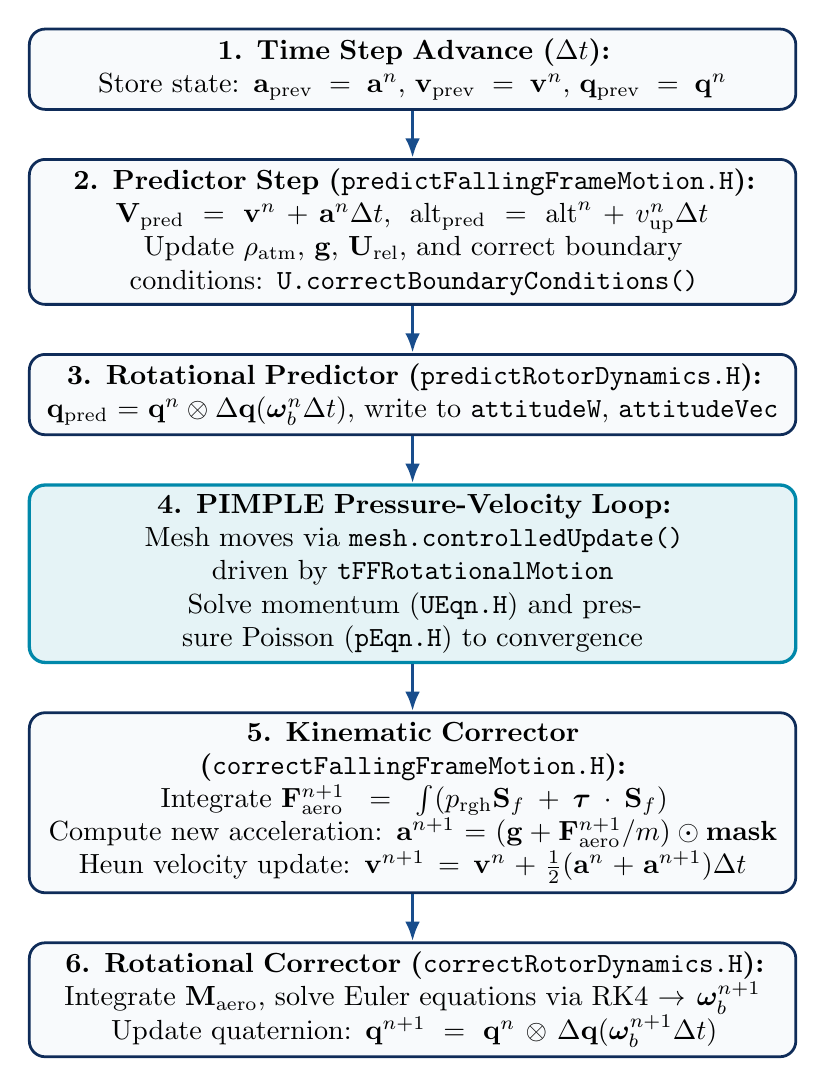
\begin{tikzpicture}[node distance=1.6cm, auto, >=Latex]
        \tikzstyle{proc} = [rectangle, draw=foamNavy, fill=foamLight, text width=9.5cm, text centered, rounded corners=2mm, minimum height=0.9cm, line width=1pt]
        \tikzstyle{loop} = [rectangle, draw=foamTeal, fill=foamTeal!10, text width=9.5cm, text centered, rounded corners=2mm, minimum height=0.9cm, line width=1.2pt]
        \tikzstyle{conn} = [draw=foamBlue, -{Latex[length=2.5mm]}, line width=1.3pt]

        \node [proc] (step1) {\textbf{1. Time Step Advance ($\Delta t$):}\\Store state: $\vect{a}_{\mathrm{prev}} = \vect{a}^n$, $\vect{v}_{\mathrm{prev}} = \vect{v}^n$, $\vect{q}_{\mathrm{prev}} = \vect{q}^n$};
        \node [proc, below=0.6cm of step1] (step2) {\textbf{2. Predictor Step (\texttt{predictFallingFrameMotion.H}):}\\$\vect{V}_{\mathrm{pred}} = \vect{v}^n + \vect{a}^n \Delta t$, \ $\mathrm{alt}_{\mathrm{pred}} = \mathrm{alt}^n + v_{\mathrm{up}}^n \Delta t$\\Update $\rho_{\mathrm{atm}}$, $\vect{g}$, $\vect{U}_{\mathrm{rel}}$, and correct boundary conditions: \texttt{U.correctBoundaryConditions()}};
        \node [proc, below=0.6cm of step2] (step3) {\textbf{3. Rotational Predictor (\texttt{predictRotorDynamics.H}):}\\$\vect{q}_{\mathrm{pred}} = \vect{q}^n \otimes \Delta \vect{q}(\omegab^n \Delta t)$, write to \texttt{attitudeW}, \texttt{attitudeVec}};
        \node [loop, below=0.6cm of step3] (step4) {\textbf{4. PIMPLE Pressure-Velocity Loop:}\\Mesh moves via \texttt{mesh.controlledUpdate()} driven by \texttt{tFFRotationalMotion}\\Solve momentum (\texttt{UEqn.H}) and pressure Poisson (\texttt{pEqn.H}) to convergence};
        \node [proc, below=0.6cm of step4] (step5) {\textbf{5. Kinematic Corrector (\texttt{correctFallingFrameMotion.H}):}\\Integrate $\faero^{n+1} = \int (\prgh \vect{S}_f + \tensor{\tau}\cdot\vect{S}_f)$\\Compute new acceleration: $\vect{a}^{n+1} = (\vect{g} + \faero^{n+1}/m) \odot \vect{mask}$\\Heun velocity update: $\vect{v}^{n+1} = \vect{v}^n + \tfrac{1}{2}(\vect{a}^n + \vect{a}^{n+1})\Delta t$};
        \node [proc, below=0.6cm of step5] (step6) {\textbf{6. Rotational Corrector (\texttt{correctRotorDynamics.H}):}\\Integrate $\maero$, solve Euler equations via RK4 $\to \omegab^{n+1}$\\Update quaternion: $\vect{q}^{n+1} = \vect{q}^n \otimes \Delta\vect{q}(\omegab^{n+1}\Delta t)$};

        \path [conn] (step1) -- (step2);
        \path [conn] (step2) -- (step3);
        \path [conn] (step3) -- (step4);
        \path [conn] (step4) -- (step5);
        \path [conn] (step5) -- (step6);
    \end{tikzpicture}
    \caption{The complete execution timeline across a single timestep $\Delta t$.}
    \label{fig:pimple_timeline}
\end{figure}

\subsection{Deep Code Inspection of Core Headers}

\subsubsection{\texttt{src/solvers/shared/createFallingFrameFields.H}}
This header parses \texttt{constant/fallingFrameDict} and registers all kinematic state fields into OpenFOAM's object registry (\texttt{mesh.thisDb()}):
\begin{lstlisting}
uniformDimensionedVectorField frameVelocity
(
    IOobject
    (
        "frameVelocity",
        runTime.timeName(),
        "uniform",
        mesh,
        IOobject::READ_IF_PRESENT,
        IOobject::AUTO_WRITE
    ),
    dimensionedVector("frameVelocity", dimVelocity, u0)
);
\end{lstlisting}
\begin{tipbox}[Why Object Registration Matters]
By specifying \texttt{IOobject::AUTO\_WRITE} and storing these fields in the \texttt{uniform/} subfolder of time directories, the simulation can be paused, stopped, or restarted from any checkpoint without losing kinetic momentum or orientation!
\end{tipbox}

\subsubsection{\texttt{src/motion/tFFRotationalMotion/tFFRotationalMotion.C}}
This is the custom \texttt{solidBodyMotionFunction} that connects the CFD mesh to the 6DoF quaternion solver:
\begin{lstlisting}
Foam::septernion Foam::solidBodyMotionFunctions::tFFRotationalMotion::transformation() const
{
    const polyMesh& mesh = time_.lookupObject<polyMesh>(polyMesh::defaultRegion);
    
    // Lookup registered quaternion fields
    const scalar w = mesh.lookupObject<uniformDimensionedScalarField>("attitudeW").value();
    const vector v = mesh.lookupObject<uniformDimensionedVectorField>("attitudeVec").value();

    quaternion q(w, v);
    q.normalise();

    // Return spatial transformation centered at hubOrigin
    return septernion(-origin_) * q * septernion(origin_);
}
\end{lstlisting}

% ============================================================================
%  SECTION 5: THE JUNIOR DEVELOPER'S PLAYBOOK
% ============================================================================
\section{The Junior Developer's Playbook: Modifying the Solver}

This is the most important section for your daily work. Follow these recipes and rules to avoid introducing critical bugs into the repository.

\subsection{Recipe 1: How to Add a New Physical Force (e.g., Thrust, Gust, or Mass Loss)}
Suppose you are assigned to model a rocket booster firing during fall, or a lateral turbulent wind gust.
Where do you insert the code?

\begin{enumerate}
    \item \textbf{Declare Configuration Keys in \texttt{createFallingFrameFields.H}:}
\begin{lstlisting}
const vector rocketThrust
(
    fallingFrameDict.getOrDefault<vector>("thrust", vector::zero)
);
\end{lstlisting}
    
    \item \textbf{Modify the Kinematic Force Balance in the Corrector Step:}\\
    Locate lines 75--85 of \texttt{correctFallingFrameMotion.H}:
\begin{lstlisting}
// Existing force balance:
gravityForce.value() = bodyMass * gravity.value();
netForce.value()     = gravityForce.value() + aeroForce.value() + rocketThrust;

vector a_new = netForce.value() / bodyMass;
a_new.x() *= freedomMask.x();
a_new.y() *= freedomMask.y();
a_new.z() *= freedomMask.z();
\end{lstlisting}

    \item \textbf{Update the Logger:} 
    Add the new force component to the 35-column logger in line 420 of \texttt{correctFallingFrameMotion.H} so it appears in \texttt{postProcessing/fallingMotion/motion.dat}.
\end{enumerate}

\subsection{Recipe 2: Modifying the PIMPLE Momentum Predictor Safely}
If you need to add custom porous drag, source terms, or buoyancy formulations to the momentum equation:
\begin{itemize}
    \item In \textbf{incompressible solvers} (\texttt{freeBodyPimpleFoam}, \texttt{freeBody6DoFPimpleFoam}), the apparent body force is absorbed into $\prgh$. Therefore, \texttt{UEqn.H} does \textbf{not} contain an explicit \texttt{fallingFrameForce} source term!
\begin{lstlisting}
tmp<fvVectorMatrix> tUEqn
(
    fvm::ddt(U) + fvm::div(phi, U)
  + MRF.DDt(U)
  + turbulence->divDevReff(U)
 ==
    fvOptions(U)
);
\end{lstlisting}
    \item In \textbf{compressible solvers} (\texttt{freeBodyRhoPimpleFoam}), the apparent force \emph{is} explicit:
\begin{lstlisting}
tmp<fvVectorMatrix> tUEqn
(
    fvm::ddt(rho, U) + fvm::div(phi, U)
  + MRF.DDt(rho, U)
  + turbulence->divDevRhoReff(U)
 ==
    fvOptions(rho, U)
  + rho * fallingFrameForce
);
\end{lstlisting}
\end{itemize}

\begin{warningbox}[Golden Rule: Keep Surface Fluxes Relative]
In moving-mesh solvers (\texttt{dynamicFvMesh}), face volume flux $\phi$ must remain \textbf{relative to mesh motion}:
\begin{lstlisting}
fvc::makeRelative(phi, U);
\end{lstlisting}
Failing to call \texttt{makeRelative} after solving pressure equations will cause continuity errors to explode to $\mathcal{O}(10^5)$ within three timesteps!
\end{warningbox}

\subsection{Crucial Traps \& Gotchas in OpenFOAM Parallel Processing}

\subsubsection{1. Parallel MPI Reductions (\texttt{reduce})}
When integrating aerodynamic forces or moments across multiple processor cores:
\begin{lstlisting}
reduce(fPress, sumOp<vector>());
reduce(fVisc,  sumOp<vector>());
reduce(mAero,  sumOp<vector>());
\end{lstlisting}
\textbf{Never omit these lines!} Without \texttt{reduce}, processor 0 only knows the forces on its local patch faces, leading to incorrect frame acceleration in parallel runs.

\subsubsection{2. Master-Only File Writing (\texttt{Pstream::master()})}
Never write to log files or disk streams without checking:
\begin{lstlisting}
if (Pstream::master())
{
    motionFile << runTime.timeName() << " " << ... << endl;
}
\end{lstlisting}
Omitting this check will cause $N$ MPI ranks to write to the same file concurrently, corrupting your simulation data!

\subsubsection{3. The \texorpdfstring{$t = 0$}{t = 0} Grid Discontinuity Trap}
When setting up an initial tilt angle for tumbling simulations:
\begin{itemize}
    \item \textbf{Wrong Way:} Specifying an initial $15^\circ$ angle in \texttt{fallingFrameDict} on an unrotated reference mesh causes \texttt{mesh.controlledUpdate()} to twist the mesh by $15^\circ$ during the very first time step $\Delta t = 10^{-5}\text{ s}$, creating an artificial grid velocity impulse of $> 400\text{ m/s}$!
    \item \textbf{Correct Way:} Physically pre-rotate the mesh geometry using OpenFOAM's transformation utility:
\begin{verbatim}
transformPoints -centre "(0 0 0)" -rotate-x 15
\end{verbatim}
    Start the simulation with attitude quaternion $\vect{q}(0) = (1, 0, 0, 0)$. Initial grid velocity is then exactly zero!
\end{itemize}

\subsection{Compilation \& Build Procedures}
The repository uses OpenFOAM's native \texttt{wmake} compilation system.

\subsubsection{Compiling the Full Suite}
From the repository root:
\begin{lstlisting}[language=bash]
./Allwmake
\end{lstlisting}
This compiles libraries and solvers in dependency order:
\begin{enumerate}
    \item \texttt{src/BCs/fallingInletVelocity} $\to$ \texttt{libfallingInletVelocity.so}
    \item \texttt{src/models/meanFlowModel} $\to$ \texttt{libfreeFallingModels.so}
    \item \texttt{src/motion/*} $\to$ \texttt{libtFFRotationalMotion.so}, \texttt{libsixDoFRotatingMotion.so}
    \item \texttt{src/solvers/*} $\to$ Executables placed into \texttt{\$FOAM\_USER\_APPBIN}
\end{enumerate}

\subsubsection{Cleaning Binaries}
\begin{lstlisting}[language=bash]
./Allwclean
\end{lstlisting}

% ============================================================================
%  SECTION 6: VERIFICATION & TESTING CHECKLIST
% ============================================================================
\section{Verification, Testing \& Diagnostics Checklist}

Before committing any modifications to Git, execute the standard verification checklist:

\subsection{Test Case 1: Steel Ball Benchmark (\texttt{steelBallRun-tFF})}
\begin{itemize}
    \item \textbf{Location:} \texttt{tutorials/steelBallRun-tFF}
    \item \textbf{Physics:} $2\text{ cm}$ steel sphere falling from rest in standard gravity ($9.81\text{ m/s}^2$).
    \item \textbf{Theoretical Terminal Velocity:} $V_t \approx 72.5\text{ m/s}$ (at $C_d \approx 0.42$).
    \item \textbf{Run Command:}
\begin{lstlisting}[language=bash]
cd tutorials/steelBallRun-tFF
./Allrun
python3 plot_motion.py
\end{lstlisting}
    \item \textbf{Verification Criteria:} Body must asymptotically approach terminal velocity; net acceleration must decay smoothly to zero without oscillations.
\end{itemize}

\subsection{Test Case 2: 6DoF Propeller Tumble (\texttt{propTumble})}
\begin{itemize}
    \item \textbf{Location:} \texttt{tutorials/propFall/cases/propTumble}
    \item \textbf{Solver:} \texttt{freeBody6DoFPimpleFoam}
    \item \textbf{Run Command (Parallel 8 Cores):}
\begin{lstlisting}[language=bash]
cd tutorials/propFall/cases/propTumble
./Allrun
python3 track_motion.py
\end{lstlisting}
    \item \textbf{Verification Criteria:} Check \texttt{postProcessing/tumbleMotion/motion.dat}. Pitch angle must develop smoothly; continuity errors must remain $< 10^{-11}$.
\end{itemize}

\begin{figure}[H]
    \centering
    \begin{subfigure}[b]{0.48\textwidth}
        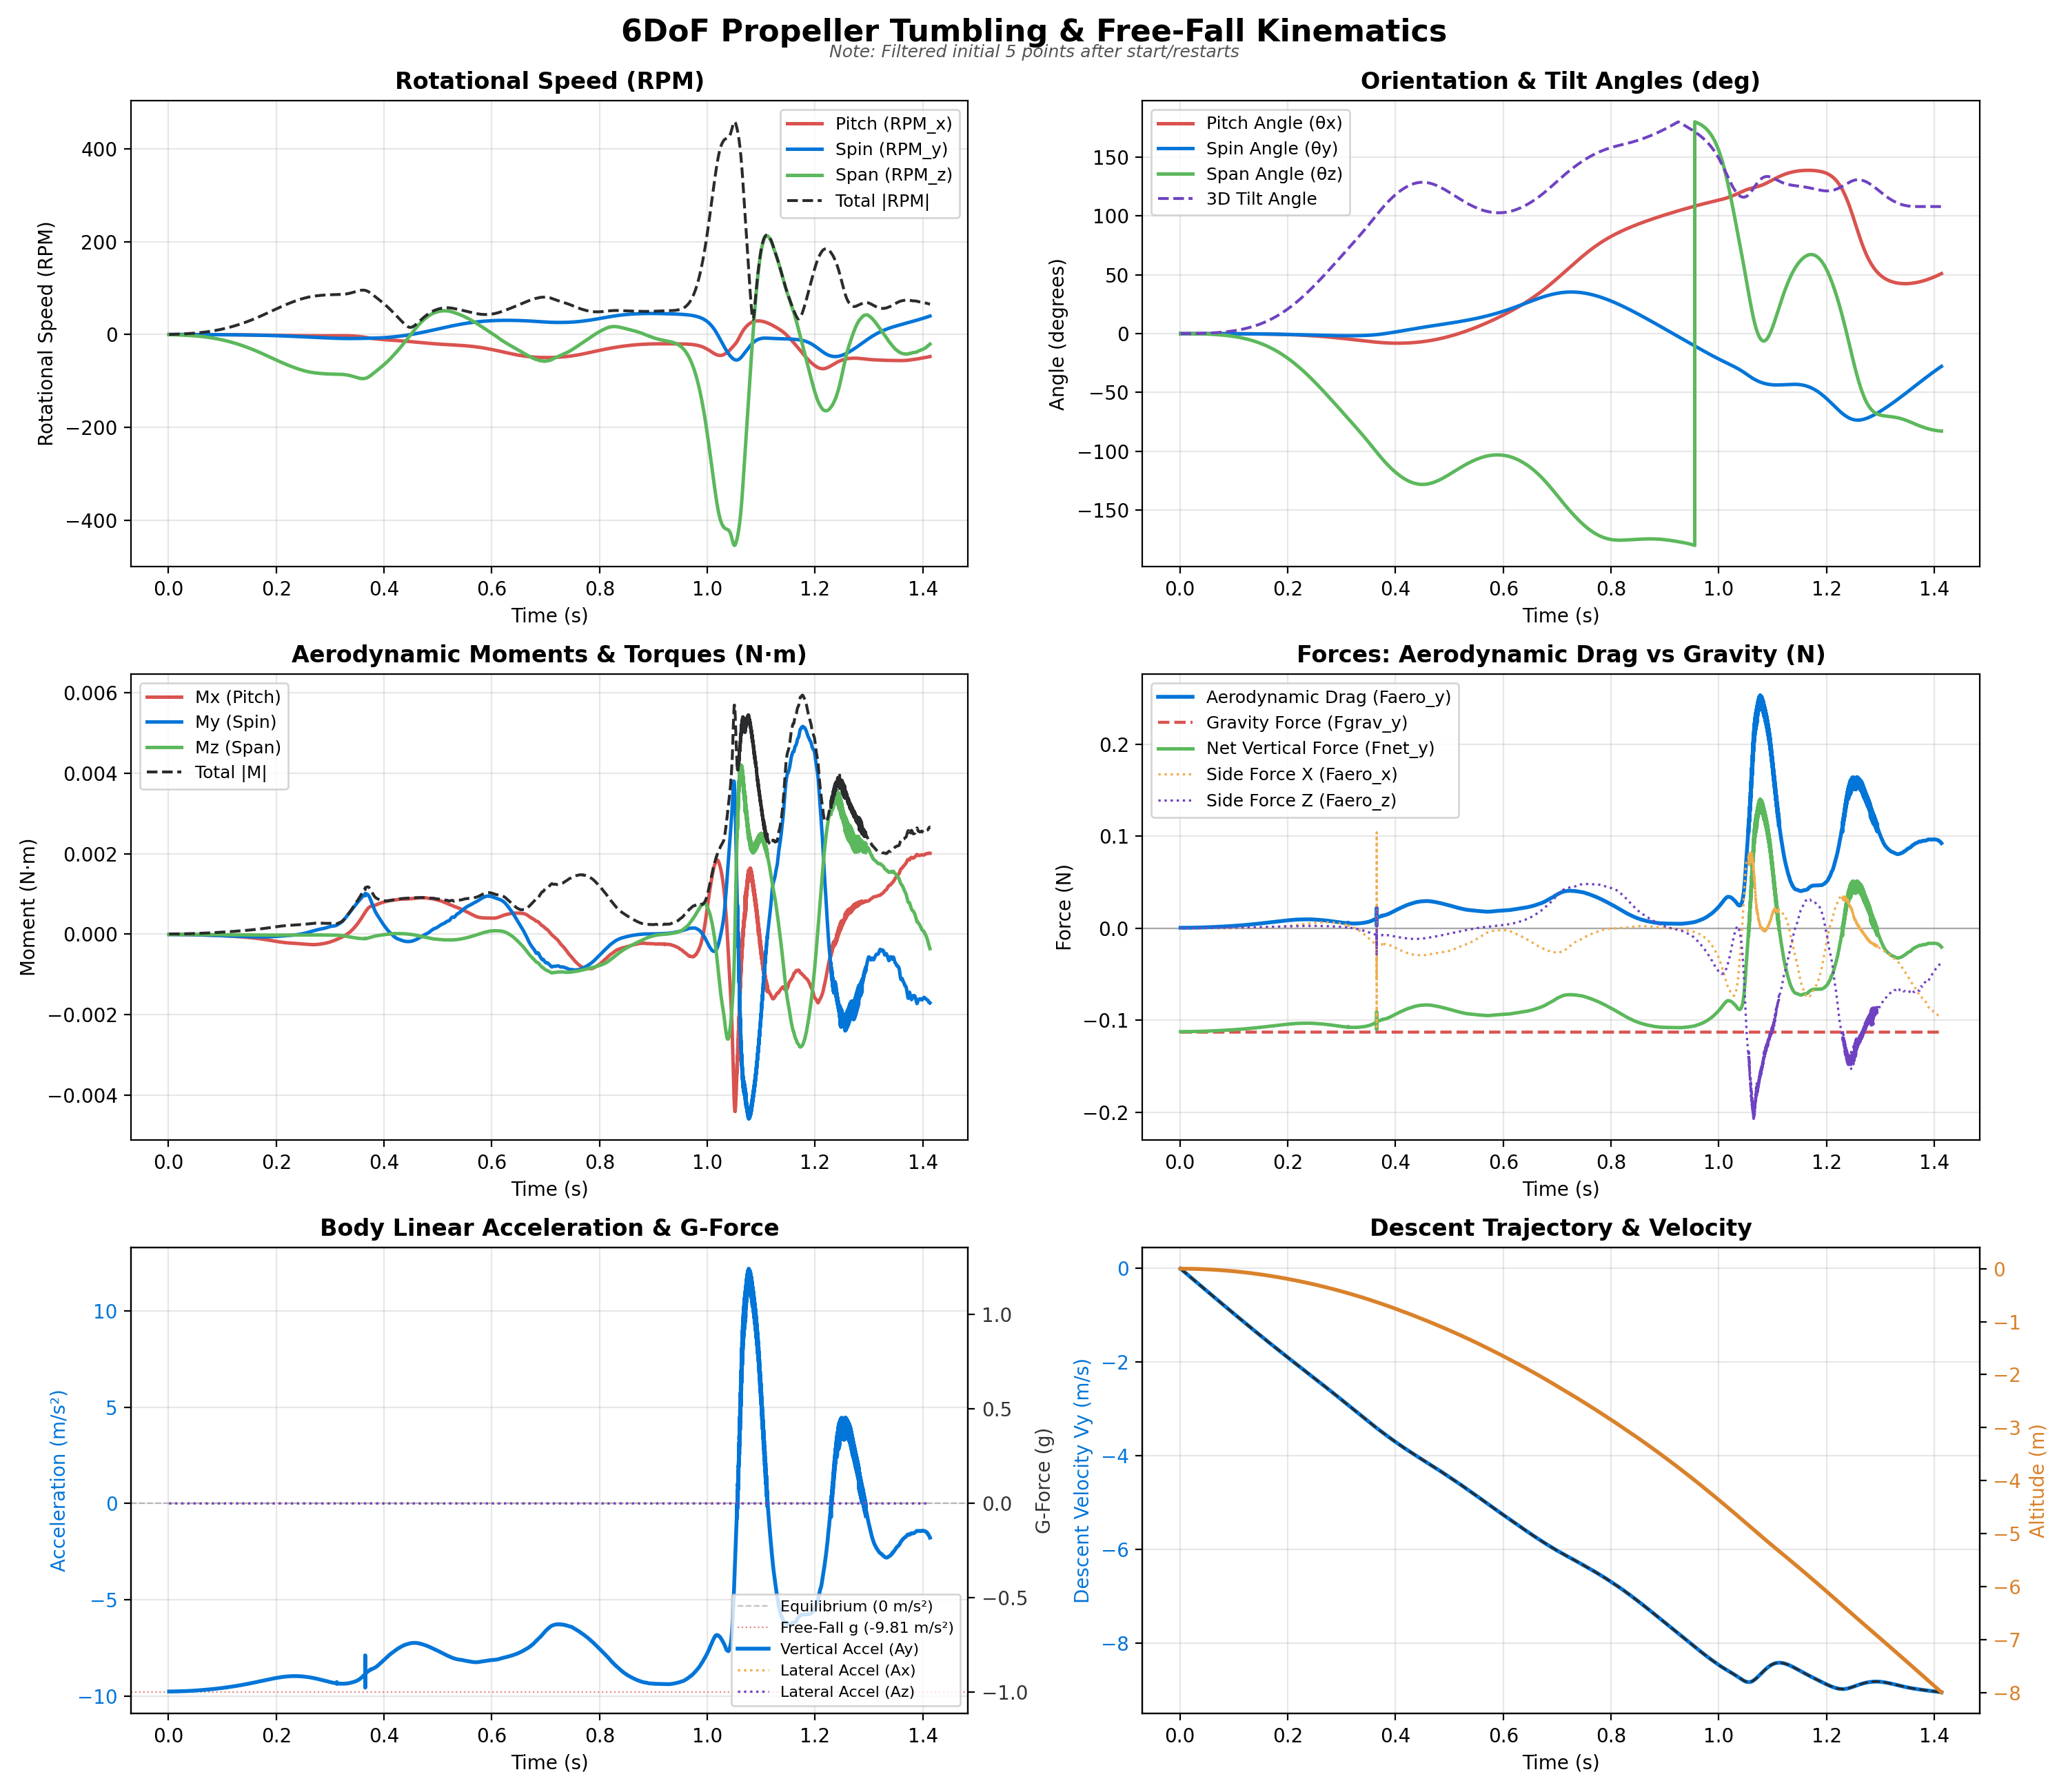
\includegraphics[width=\textwidth]{figures/motion_tracking_report.png}
        \caption{6DoF Tumbling Kinematics Tracked in \texttt{propTumble}.}
    \end{subfigure}
    \hfill
    \begin{subfigure}[b]{0.48\textwidth}
        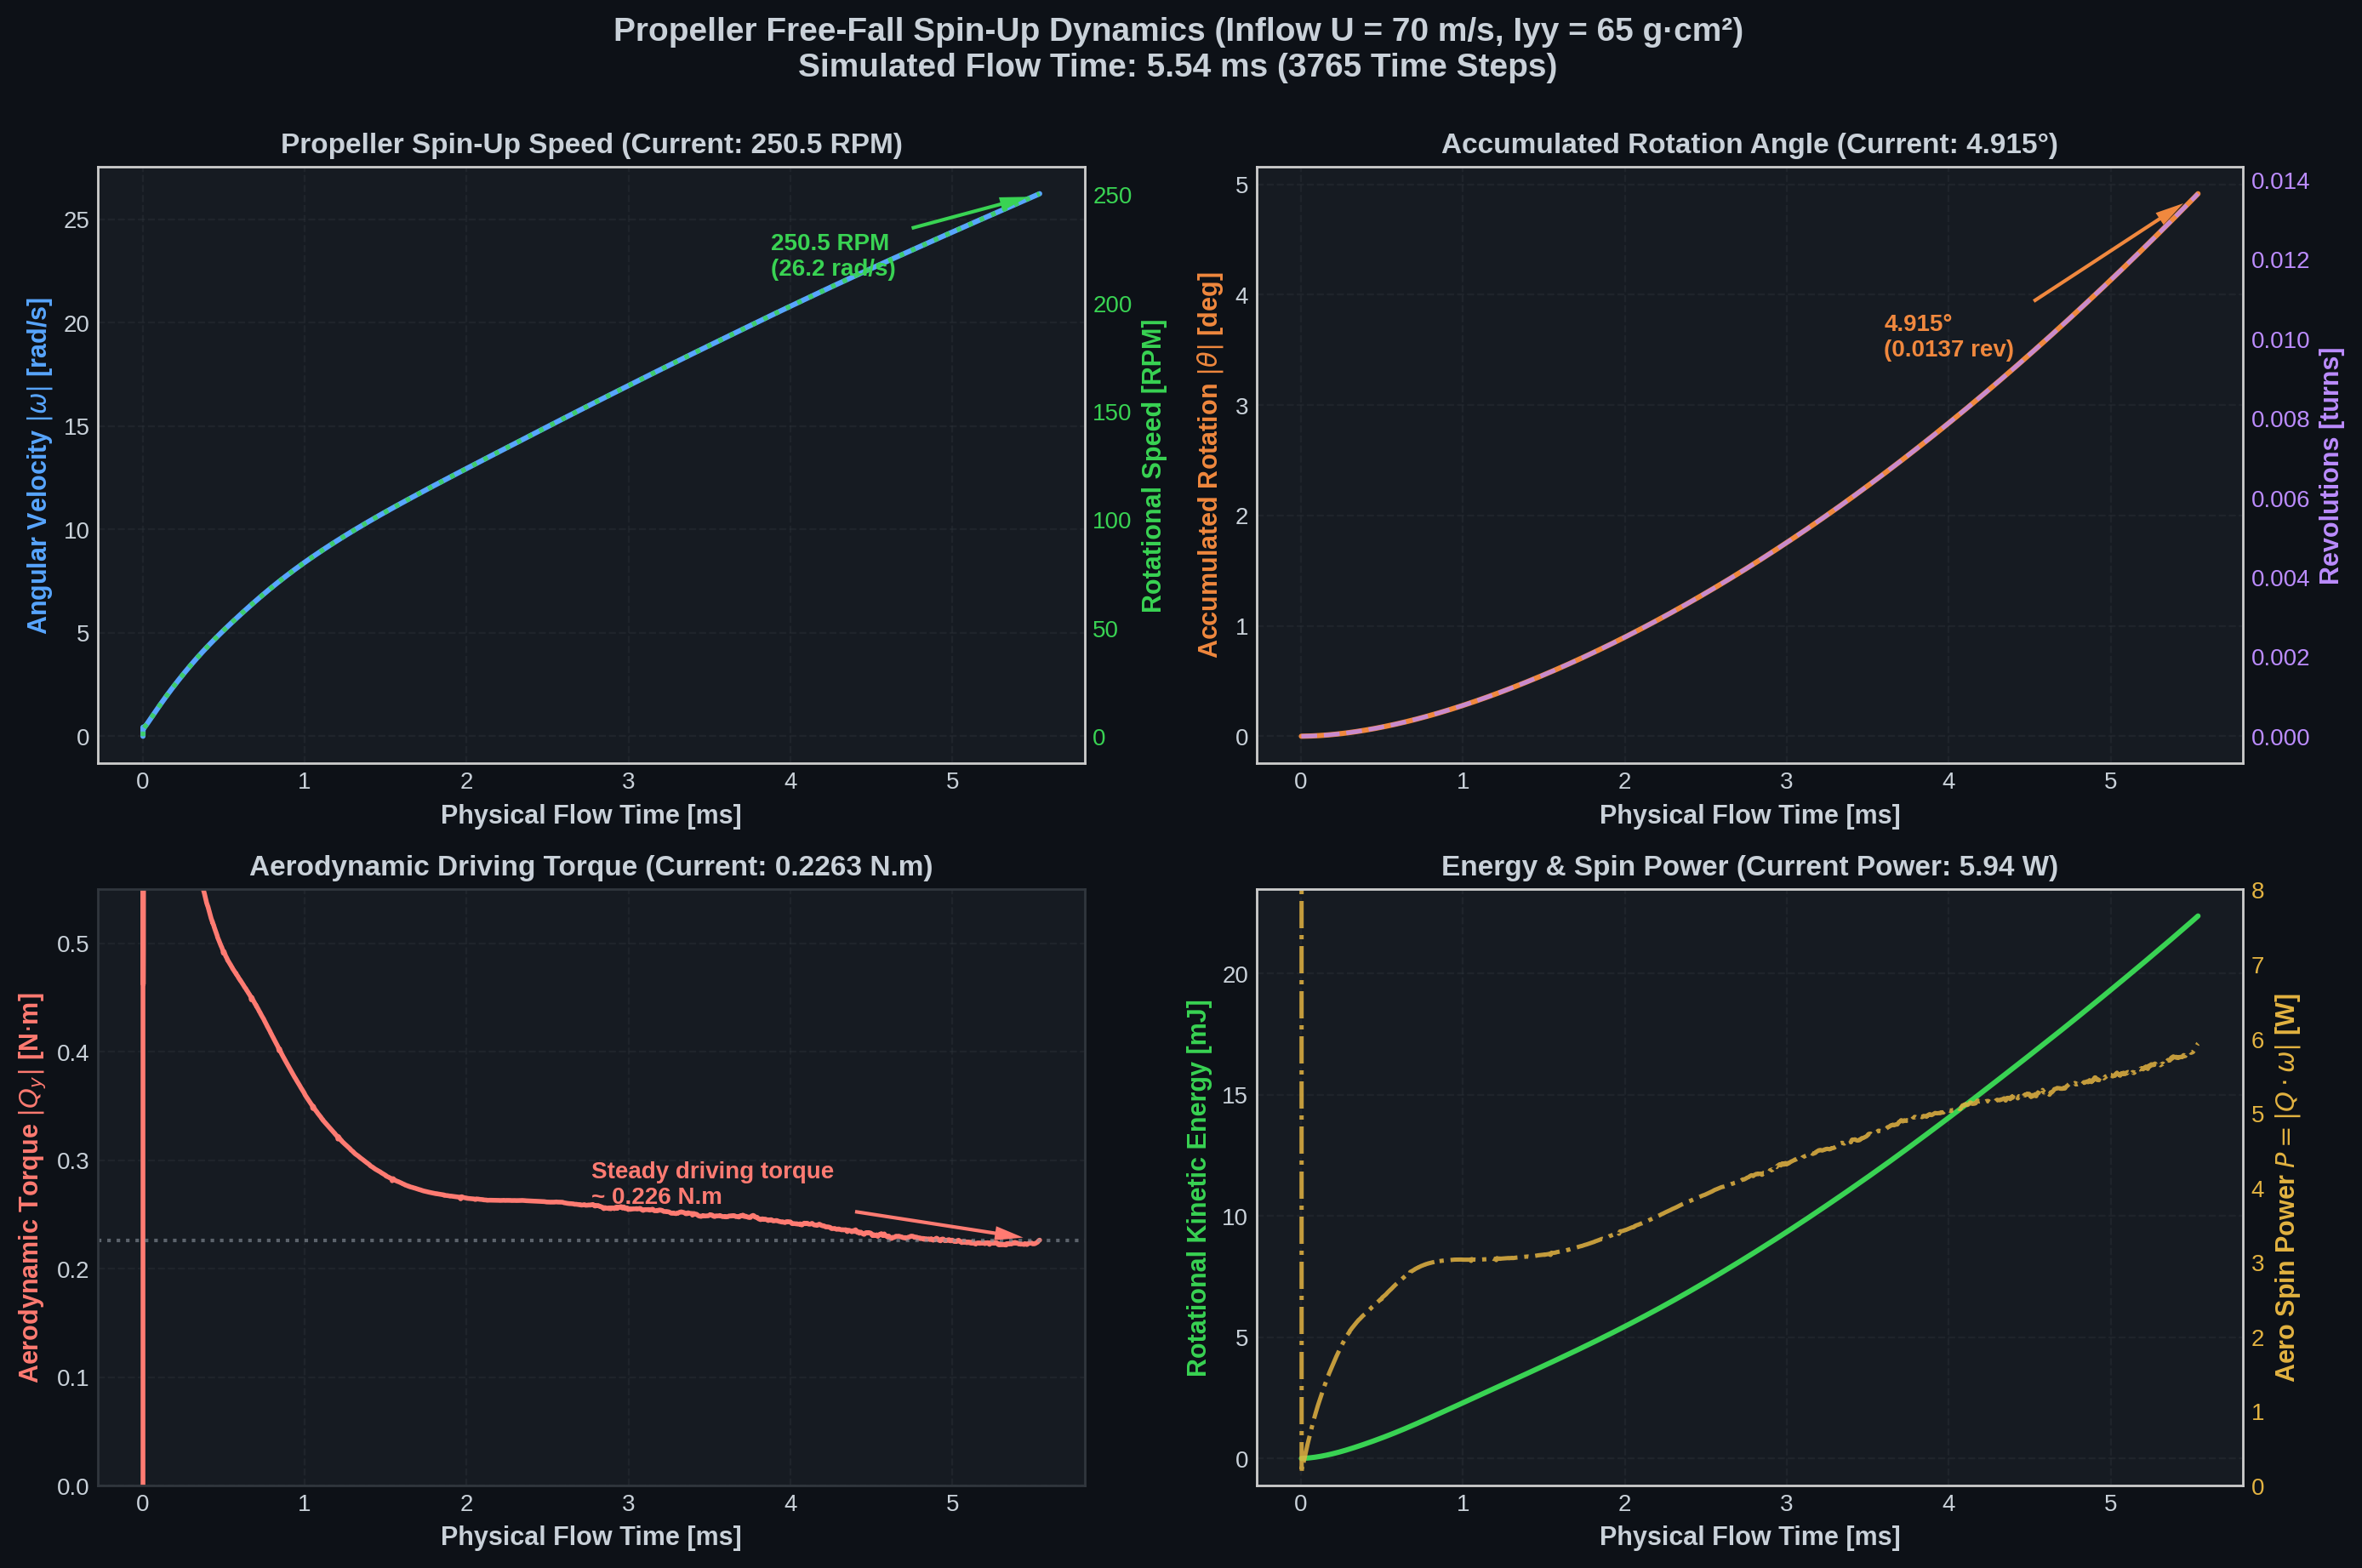
\includegraphics[width=\textwidth]{figures/rotation_plot.png}
        \caption{Angular Velocity Evolution across Principal Axes.}
    \end{subfigure}
    \caption{Experimental simulation outputs from the verification suite.}
    \label{fig:verification_plots}
\end{figure}

% ============================================================================
%  SECTION 7: DEVELOPER'S QUICK REFERENCE SHEET
% ============================================================================
\section{Developer's Quick Reference Guide}

\begin{table}[H]
    \centering
    \small
    \caption{Key Solver Variables in \texttt{src/solvers/shared/createFallingFrameFields.H}.}
    \label{tab:quick_ref}
    \begin{tabularx}{\textwidth}{l l l X}
        \toprule
        \textbf{C++ Variable} & \textbf{OpenFOAM Object Name} & \textbf{Dimensions} & \textbf{Description} \\
        \midrule
        \texttt{frameVelocity} & \texttt{"frameVelocity"} & $[0\ 1\ -1\ 0\ 0\ 0\ 0]$ & Kinematic frame velocity vector $\vframe(t)$. \\
        \texttt{frameAcceleration} & \texttt{"frameAcceleration"} & $[0\ 1\ -2\ 0\ 0\ 0\ 0]$ & Instantaneous acceleration vector $\aframe(t)$. \\
        \texttt{altitude} & \texttt{"altitude"} & $[0\ 1\ 0\ 0\ 0\ 0\ 0]$ & Tracked physical altitude $z(t)$ above ground. \\
        \texttt{fallingFrameForce} & \texttt{"fallingFrameForce"} & $[0\ 1\ -2\ 0\ 0\ 0\ 0]$ & Apparent body force vector $\vect{g} - \aframe(t)$. \\
        \texttt{relativeVelocity} & \texttt{"relativeVelocity"} & $[0\ 1\ -1\ 0\ 0\ 0\ 0]$ & Freestream inflow vector $\vect{U}_{\mathrm{mean}} - \vframe(t)$. \\
        \texttt{attitudeW} & \texttt{"attitudeW"} & $[0\ 0\ 0\ 0\ 0\ 0\ 0]$ & Scalar component $q_w$ of attitude quaternion. \\
        \texttt{attitudeVec} & \texttt{"attitudeVec"} & $[0\ 0\ 0\ 0\ 0\ 0\ 0]$ & Vector part $(q_x, q_y, q_z)$ of attitude quaternion. \\
        \texttt{angularVelocity} & \texttt{"angularVelocity"} & $[0\ 0\ -1\ 0\ 0\ 0\ 0]$ & Angular velocity $\omegab$ in body frame [rad/s]. \\
        \texttt{aeroMoment} & \texttt{"aeroMoment"} & $[1\ 2\ -2\ 0\ 0\ 0\ 0]$ & Aerodynamic torque $\maero$ in world frame [$\text{N}\cdot\text{m}$]. \\
        \bottomrule
    \end{tabularx}
\end{table}

\section*{Summary \& Closing Words}
You are now equipped with the mathematical, algorithmic, and practical knowledge required to develop within the \texttt{freeFallingFoam} ecosystem. Remember:
\begin{itemize}
    \item Always respect the Heun predictor-corrector sequence.
    \item Never compute aerodynamic moments on raw static pressure $p$ in incompressible solvers; use $\prgh$.
    \item Maintain parallel reduction safety on all integrated quantities.
\end{itemize}
Welcome aboard, and happy coding!

\end{document}
